\documentclass{article}%
\usepackage[T1]{fontenc}%
\usepackage[utf8]{inputenc}%
\usepackage{lmodern}%
\usepackage{textcomp}%
\usepackage{lastpage}%
\usepackage[head=40pt,margin=0.5in,bottom=0.6in]{geometry}%
\usepackage{graphicx}%
%
\title{\textbf{110 yupkas dejaron la Sierra de Perijá y se instalaron en Cúcuta}}%
\author{El Nacional Web}%
\date{06/10/2018}%
%
\begin{document}%
\normalsize%
\maketitle%
\textbf{URL: }%
http://www.el{-}nacional.com/noticias/sociedad/110{-}yupkas{-}dejaron{-}sierra{-}perija{-}instalaron{-}cucuta\_254636\newline%
%
\textbf{Periodico: }%
EN, %
ID: %
254636, %
Seccion: %
Sociedad\newline%
%
\textbf{Palabras Claves: }%
Diáspora, Zulia, Sociedad\newline%
%
\textbf{Derecho: }%
2.9, %
Otros Derechos: %
2.10, %
Sub Derechos: %
2.9.1, 2.10.1\newline%
%
\textbf{EP: }%
NO\newline%
\newline%
%
\textbf{\textit{Los oriundos del estado Zulia solo comían una vez al día cada dos días cuando estaban en Venezuela~}}%
\newline%
\newline%
%
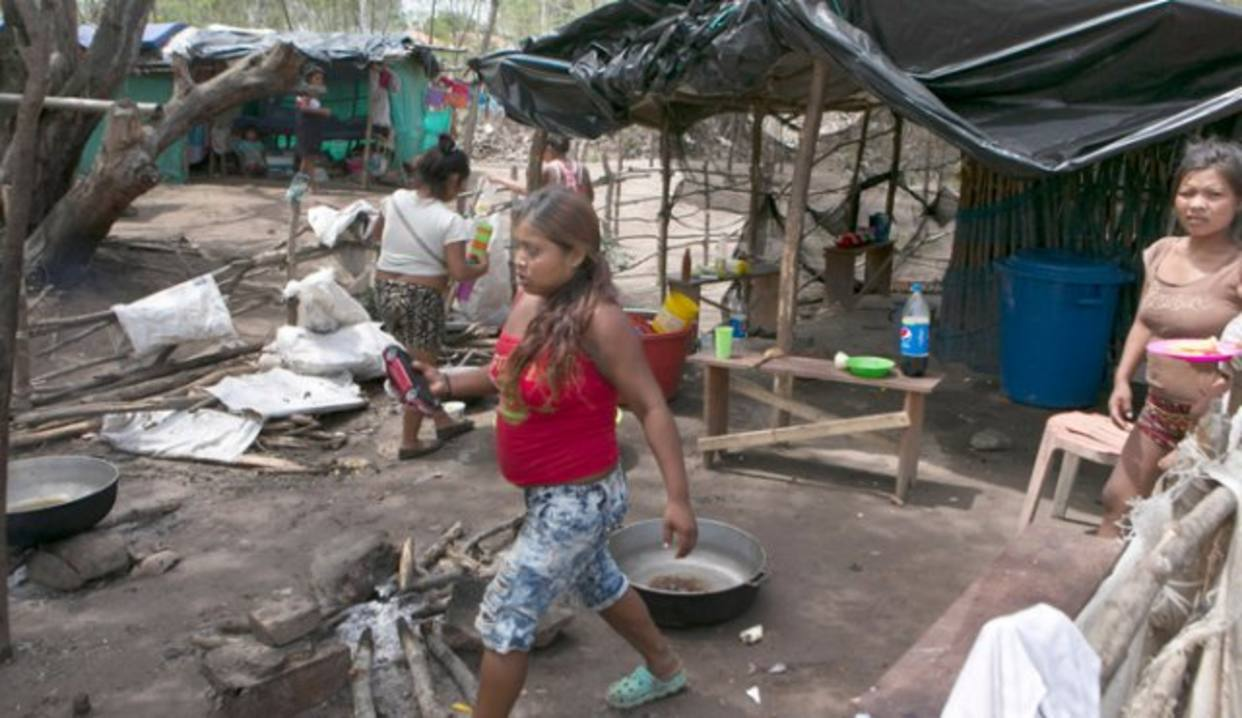
\includegraphics[width=300px]{61.jpg}%
\newline%
%
Al menos 110 yukpas, oriundos de la Sierra de Perijá en el estado Zulia, decidieron cruzar la frontera hacía Cúcuta para sortear las dificultades económicas que padecían en Venezuela.%
\newline%
%
“Allá llegamos al extremo de comer solo una ración cada dos días, y ello nos tenía muy preocupados, por los niños”, dijo Dionisio Finol, jefe del grupo yukpa que se ubica a orillas del río Táchira en El Escobal, reseñó~La Opinión~de Cúcuta.%
\newline%
%
Finol resaltó que no tiene planeado regresar a Venezuela porque “no queremos que nuestra comunidad pase penurias”.%
\newline%
%
110 personas, entre ellos 62 niños, dejaron la Sierra y se instalaron en Cúcuta enfrentaron dificultades de salud al llegar a El Escobal.%
\newline%
%
“Gracias a Cruz Roja Internacional y a Acnur, nuestros niños recibieron medicinas y recobraron la salud. También, ahora, tenemos tres raciones de comida diarias para todos”, detalló Finol.%
\newline%
%
Leer más en~La Opinión%
\newline%
%
\end{document}